% Options for packages loaded elsewhere
% Options for packages loaded elsewhere
\PassOptionsToPackage{unicode}{hyperref}
\PassOptionsToPackage{hyphens}{url}
\PassOptionsToPackage{dvipsnames,svgnames,x11names}{xcolor}
%
\documentclass[
  letterpaper,
  DIV=11,
  numbers=noendperiod]{scrreprt}
\usepackage{xcolor}
\usepackage{amsmath,amssymb}
\setcounter{secnumdepth}{5}
\usepackage{iftex}
\ifPDFTeX
  \usepackage[T1]{fontenc}
  \usepackage[utf8]{inputenc}
  \usepackage{textcomp} % provide euro and other symbols
\else % if luatex or xetex
  \usepackage{unicode-math} % this also loads fontspec
  \defaultfontfeatures{Scale=MatchLowercase}
  \defaultfontfeatures[\rmfamily]{Ligatures=TeX,Scale=1}
\fi
\usepackage{lmodern}
\ifPDFTeX\else
  % xetex/luatex font selection
\fi
% Use upquote if available, for straight quotes in verbatim environments
\IfFileExists{upquote.sty}{\usepackage{upquote}}{}
\IfFileExists{microtype.sty}{% use microtype if available
  \usepackage[]{microtype}
  \UseMicrotypeSet[protrusion]{basicmath} % disable protrusion for tt fonts
}{}
\makeatletter
\@ifundefined{KOMAClassName}{% if non-KOMA class
  \IfFileExists{parskip.sty}{%
    \usepackage{parskip}
  }{% else
    \setlength{\parindent}{0pt}
    \setlength{\parskip}{6pt plus 2pt minus 1pt}}
}{% if KOMA class
  \KOMAoptions{parskip=half}}
\makeatother
% Make \paragraph and \subparagraph free-standing
\makeatletter
\ifx\paragraph\undefined\else
  \let\oldparagraph\paragraph
  \renewcommand{\paragraph}{
    \@ifstar
      \xxxParagraphStar
      \xxxParagraphNoStar
  }
  \newcommand{\xxxParagraphStar}[1]{\oldparagraph*{#1}\mbox{}}
  \newcommand{\xxxParagraphNoStar}[1]{\oldparagraph{#1}\mbox{}}
\fi
\ifx\subparagraph\undefined\else
  \let\oldsubparagraph\subparagraph
  \renewcommand{\subparagraph}{
    \@ifstar
      \xxxSubParagraphStar
      \xxxSubParagraphNoStar
  }
  \newcommand{\xxxSubParagraphStar}[1]{\oldsubparagraph*{#1}\mbox{}}
  \newcommand{\xxxSubParagraphNoStar}[1]{\oldsubparagraph{#1}\mbox{}}
\fi
\makeatother


\usepackage{longtable,booktabs,array}
\newcounter{none} % for unnumbered tables
\usepackage{calc} % for calculating minipage widths
% Correct order of tables after \paragraph or \subparagraph
\usepackage{etoolbox}
\makeatletter
\patchcmd\longtable{\par}{\if@noskipsec\mbox{}\fi\par}{}{}
\makeatother
% Allow footnotes in longtable head/foot
\IfFileExists{footnotehyper.sty}{\usepackage{footnotehyper}}{\usepackage{footnote}}
\makesavenoteenv{longtable}
\usepackage{graphicx}
\makeatletter
\newsavebox\pandoc@box
\newcommand*\pandocbounded[1]{% scales image to fit in text height/width
  \sbox\pandoc@box{#1}%
  \Gscale@div\@tempa{\textheight}{\dimexpr\ht\pandoc@box+\dp\pandoc@box\relax}%
  \Gscale@div\@tempb{\linewidth}{\wd\pandoc@box}%
  \ifdim\@tempb\p@<\@tempa\p@\let\@tempa\@tempb\fi% select the smaller of both
  \ifdim\@tempa\p@<\p@\scalebox{\@tempa}{\usebox\pandoc@box}%
  \else\usebox{\pandoc@box}%
  \fi%
}
% Set default figure placement to htbp
\def\fps@figure{htbp}
\makeatother

\ifLuaTeX
  \usepackage{luacolor}
  \usepackage[soul]{lua-ul}
\else
  \usepackage{soul}
\fi




\setlength{\emergencystretch}{3em} % prevent overfull lines

\providecommand{\tightlist}{%
  \setlength{\itemsep}{0pt}\setlength{\parskip}{0pt}}



 


\KOMAoption{captions}{tableheading}
\makeatletter
\@ifpackageloaded{tcolorbox}{}{\usepackage[skins,breakable]{tcolorbox}}
\@ifpackageloaded{fontawesome5}{}{\usepackage{fontawesome5}}
\definecolor{quarto-callout-color}{HTML}{909090}
\definecolor{quarto-callout-note-color}{HTML}{0758E5}
\definecolor{quarto-callout-important-color}{HTML}{CC1914}
\definecolor{quarto-callout-warning-color}{HTML}{EB9113}
\definecolor{quarto-callout-tip-color}{HTML}{00A047}
\definecolor{quarto-callout-caution-color}{HTML}{FC5300}
\definecolor{quarto-callout-color-frame}{HTML}{acacac}
\definecolor{quarto-callout-note-color-frame}{HTML}{4582ec}
\definecolor{quarto-callout-important-color-frame}{HTML}{d9534f}
\definecolor{quarto-callout-warning-color-frame}{HTML}{f0ad4e}
\definecolor{quarto-callout-tip-color-frame}{HTML}{02b875}
\definecolor{quarto-callout-caution-color-frame}{HTML}{fd7e14}
\makeatother
\makeatletter
\@ifpackageloaded{bookmark}{}{\usepackage{bookmark}}
\makeatother
\makeatletter
\@ifpackageloaded{caption}{}{\usepackage{caption}}
\AtBeginDocument{%
\ifdefined\contentsname
  \renewcommand*\contentsname{Table of contents}
\else
  \newcommand\contentsname{Table of contents}
\fi
\ifdefined\listfigurename
  \renewcommand*\listfigurename{List of Figures}
\else
  \newcommand\listfigurename{List of Figures}
\fi
\ifdefined\listtablename
  \renewcommand*\listtablename{List of Tables}
\else
  \newcommand\listtablename{List of Tables}
\fi
\ifdefined\figurename
  \renewcommand*\figurename{Figure}
\else
  \newcommand\figurename{Figure}
\fi
\ifdefined\tablename
  \renewcommand*\tablename{Table}
\else
  \newcommand\tablename{Table}
\fi
}
\@ifpackageloaded{float}{}{\usepackage{float}}
\floatstyle{ruled}
\@ifundefined{c@chapter}{\newfloat{codelisting}{h}{lop}}{\newfloat{codelisting}{h}{lop}[chapter]}
\floatname{codelisting}{Listing}
\newcommand*\listoflistings{\listof{codelisting}{List of Listings}}
\makeatother
\makeatletter
\makeatother
\makeatletter
\@ifpackageloaded{caption}{}{\usepackage{caption}}
\@ifpackageloaded{subcaption}{}{\usepackage{subcaption}}
\makeatother
\newcounter{quartocallouttipno}
\newcommand{\quartocallouttip}[1]{\refstepcounter{quartocallouttipno}\label{#1}}
\usepackage{bookmark}
\IfFileExists{xurl.sty}{\usepackage{xurl}}{} % add URL line breaks if available
\urlstyle{same}
\hypersetup{
  pdftitle={An Introduction to Errors and Error Analysis},
  pdfauthor={Fiona Dickinson},
  colorlinks=true,
  linkcolor={blue},
  filecolor={Maroon},
  citecolor={Blue},
  urlcolor={Blue},
  pdfcreator={LaTeX via pandoc}}


\title{An Introduction to Errors and Error Analysis}
\author{Fiona Dickinson}
\date{2026-06-15}
\begin{document}
\maketitle

\renewcommand*\contentsname{Table of contents}
{
\setcounter{tocdepth}{2}
\tableofcontents
}

\bookmarksetup{startatroot}

\chapter*{Introduction}\label{sec-introduction}
\addcontentsline{toc}{chapter}{Introduction}

\markboth{Introduction}{Introduction}

This resource is created to scaffold your learning of errors and
uncertainty in data analysis. Whilst these skills are taught here away
from the lab, it is usually in the physical and analytical laboratory
setting where you will use these skills.

The resource is written in Markdown and has embedded questions which
provide feedback. It is strongly encouraged that you start at the
beginning and work through on your first use to check your learning.
However you should be able to refer to sections as required when you are
more familiar with the content.

The resource contains a number of `highlight blocks'.

\begin{tcolorbox}[enhanced jigsaw, arc=.35mm, bottomrule=.15mm, bottomtitle=1mm, breakable, colback=white, colbacktitle=quarto-callout-tip-color!10!white, colframe=quarto-callout-tip-color-frame, coltitle=black, left=2mm, leftrule=.75mm, opacityback=0, opacitybacktitle=0.6, rightrule=.15mm, title=\textcolor{quarto-callout-tip-color}{\faLightbulb}\hspace{0.5em}{Green blocks contain our `rules' for handling significant figures and
errors.}, titlerule=0mm, toprule=.15mm, toptitle=1mm]

The rules may appear as text or equations.

\end{tcolorbox}

\begin{tcolorbox}[enhanced jigsaw, arc=.35mm, bottomrule=.15mm, bottomtitle=1mm, breakable, colback=white, colbacktitle=quarto-callout-caution-color!10!white, colframe=quarto-callout-caution-color-frame, coltitle=black, left=2mm, leftrule=.75mm, opacityback=0, opacitybacktitle=0.6, rightrule=.15mm, title=\textcolor{quarto-callout-caution-color}{\faFire}\hspace{0.5em}{Orange blocks contain worked example questions.}, titlerule=0mm, toprule=.15mm, toptitle=1mm]

The question followed by commented worked solutions should help you
clarify concepts.

\end{tcolorbox}

\begin{tcolorbox}[enhanced jigsaw, arc=.35mm, bottomrule=.15mm, bottomtitle=1mm, breakable, colback=white, colbacktitle=quarto-callout-note-color!10!white, colframe=quarto-callout-note-color-frame, coltitle=black, left=2mm, leftrule=.75mm, opacityback=0, opacitybacktitle=0.6, rightrule=.15mm, title=\textcolor{quarto-callout-note-color}{\faInfo}\hspace{0.5em}{Blue blocks contain questions for you to try. Press the arrow.}, titlerule=0mm, toprule=.15mm, toptitle=1mm]

Blue blocks will always have the answer `hidden' in the drop down.
Please attempt questions before accessing the drop down, writing down
your answer.

Why? because writing it down make you commit, and if you get it wrong
you will think more about why you got it wrong.

\end{tcolorbox}

\begin{tcolorbox}[enhanced jigsaw, arc=.35mm, bottomrule=.15mm, bottomtitle=1mm, breakable, colback=white, colbacktitle=quarto-callout-important-color!10!white, colframe=quarto-callout-important-color-frame, coltitle=black, left=2mm, leftrule=.75mm, opacityback=0, opacitybacktitle=0.6, rightrule=.15mm, title=\textcolor{quarto-callout-important-color}{\faExclamation}\hspace{0.5em}{Red blocks contain warnings.}, titlerule=0mm, toprule=.15mm, toptitle=1mm]

These may be observations about common student errors, or
misconceptions.

\end{tcolorbox}

Chapter Chapter~\ref{sec-chapter1}

\begin{itemize}
\tightlist
\item
  Section~\ref{sec-precisionaccuracy} Understanding precision and
  accuracy.
\item
  Section~\ref{sec-significantfigures} Understanding significant figures
  and how to count them.
\item
  Section~\ref{sec-howmanysf} How many significant figures are there?
\item
  Section~\ref{sec-readingvalues} Making measurements and reading
  scales.
\item
  Section~\ref{sec-roundtoeven} Rounding to even.
\end{itemize}

Chapter Chapter~\ref{sec-chapter2}

\begin{itemize}
\tightlist
\item
  Section~\ref{sec-sfaddsub} Using significant figures in addition and
  subtraction.
\item
  Section~\ref{sec-sfmuldiv} Using significant figures in multiplication
  and division.
\item
  Section~\ref{sec-sflog} Using significant figures with logs.
\item
  \textbf{?@sec-sfpowers} Using significant figures with powers and
  roots.
\item
  \textbf{?@sec-sfmixed} Using significant figures in mixed
  calculations.
\end{itemize}

Chapter 3: Averages and Standard Deviation

\begin{itemize}
\tightlist
\item
  Calculating averages to appropriate significant figures.
\item
  Understanding data distribution and standard deviation.
\end{itemize}

Chapter 4: The Standard Error

\begin{itemize}
\tightlist
\item
  The standard error, a measure of our confidence in the sample mean.
\item
  Use of significant figures in reporting the standard error and the
  mean.
\end{itemize}

Chapter 5: The Standard Error of Gradients and Intercepts

\begin{itemize}
\tightlist
\item
  Calculating the standard error of gradients and intercepts in linear
  regression.
\item
  Examples in Excel.
\item
  Examples in Python.
\end{itemize}

\section*{Resource Credits}\label{resource-credits}
\addcontentsline{toc}{section}{Resource Credits}

\markright{Resource Credits}

This resource was created in conjunction with MAST at the University of
Bath. Thanks go to Dr Tamsin Smith and in particular Ed Southwood for
considerable assistance in developing the code for the regenerative
questions.

This workbook works in conjunction with Chapters 2 and 3 of
\href{https://books.rsc.org/books/monograph/1959/Introduction-to-Contextual-Maths-in-Chemistry}{``An
Introduction to Contextual Maths in Chemistry'' by Fiona Dickinson and
Andrew McKinley}, which is available in
\href{https://bath.primo.exlibrisgroup.com/discovery/fulldisplay?docid=alma991003768059702761&context=L&vid=44BAT_INST:44BAT_VU1&lang=en&search_scope=MyInst_and_CI&adaptor=Local\%20Search\%20Engine&isFrbr=true&tab=Everything&query=any,contains,maths\%20dickinson&sortby=date_d&facet=frbrgroupid,include,9045141419038150349&offset=0}{paper}
and
\href{https://bath.primo.exlibrisgroup.com/discovery/fulldisplay?docid=alma991003857104302761&context=L&vid=44BAT_INST:44BAT_VU1&lang=en&search_scope=MyInst_and_CI&adaptor=Local\%20Search\%20Engine&isFrbr=true&tab=Everything&query=any,contains,maths\%20dickinson&sortby=date_d&facet=frbrgroupid,include,9045141419038150349&offset=0}{digital
form} from the University of Bath library.

\section*{Error reporting}\label{error-reporting}
\addcontentsline{toc}{section}{Error reporting}

\markright{Error reporting}

Whilst care is taken in production of this manuscript, errors may be
present. If you find an error, please report using the form below. Thank
you for your help in improving this resource.

\section*{Resource history}\label{resource-history}
\addcontentsline{toc}{section}{Resource history}

\markright{Resource history}

\begin{itemize}
\tightlist
\item
  30th July 2026 - Chapter 2 SAQ included.
\item
  17th July 2026 - First embedded question code included, chapter 2
  start.
\item
  16th June 2026 - First commit of index and chapter 1.
\end{itemize}

\bookmarksetup{startatroot}

\chapter{How many significant figures are there?}\label{sec-chapter1}

\section{Before we begin\ldots{} Precision and
Accuracy.}\label{sec-precisionaccuracy}

In talking about significant figures, standard erro and propagation of
error, we need to be clear about what we mean by precision and accuracy.

Data has a spread, in taking physical measurements this is not something
we can avoid. How well we can record a value is frequently limited by
the equipment we are using. We will talk more about this spread of data
in later chapters of this resource.

\begin{tcolorbox}[enhanced jigsaw, arc=.35mm, bottomrule=.15mm, bottomtitle=1mm, breakable, colback=white, colbacktitle=quarto-callout-tip-color!10!white, colframe=quarto-callout-tip-color-frame, coltitle=black, left=2mm, leftrule=.75mm, opacityback=0, opacitybacktitle=0.6, rightrule=.15mm, title=\textcolor{quarto-callout-tip-color}{\faLightbulb}\hspace{0.5em}{Tip \ref*{tip-accuracyandprecision}}, titlerule=0mm, toprule=.15mm, toptitle=1mm]

\quartocallouttip{tip-accuracyandprecision} 

\begin{itemize}
\tightlist
\item
  Accuracy is how close a measurement is to the true value.
\item
  Precision is how close a set of measurements are to each other.
\end{itemize}

\end{tcolorbox}

\begin{figure}[H]

{\centering \pandocbounded{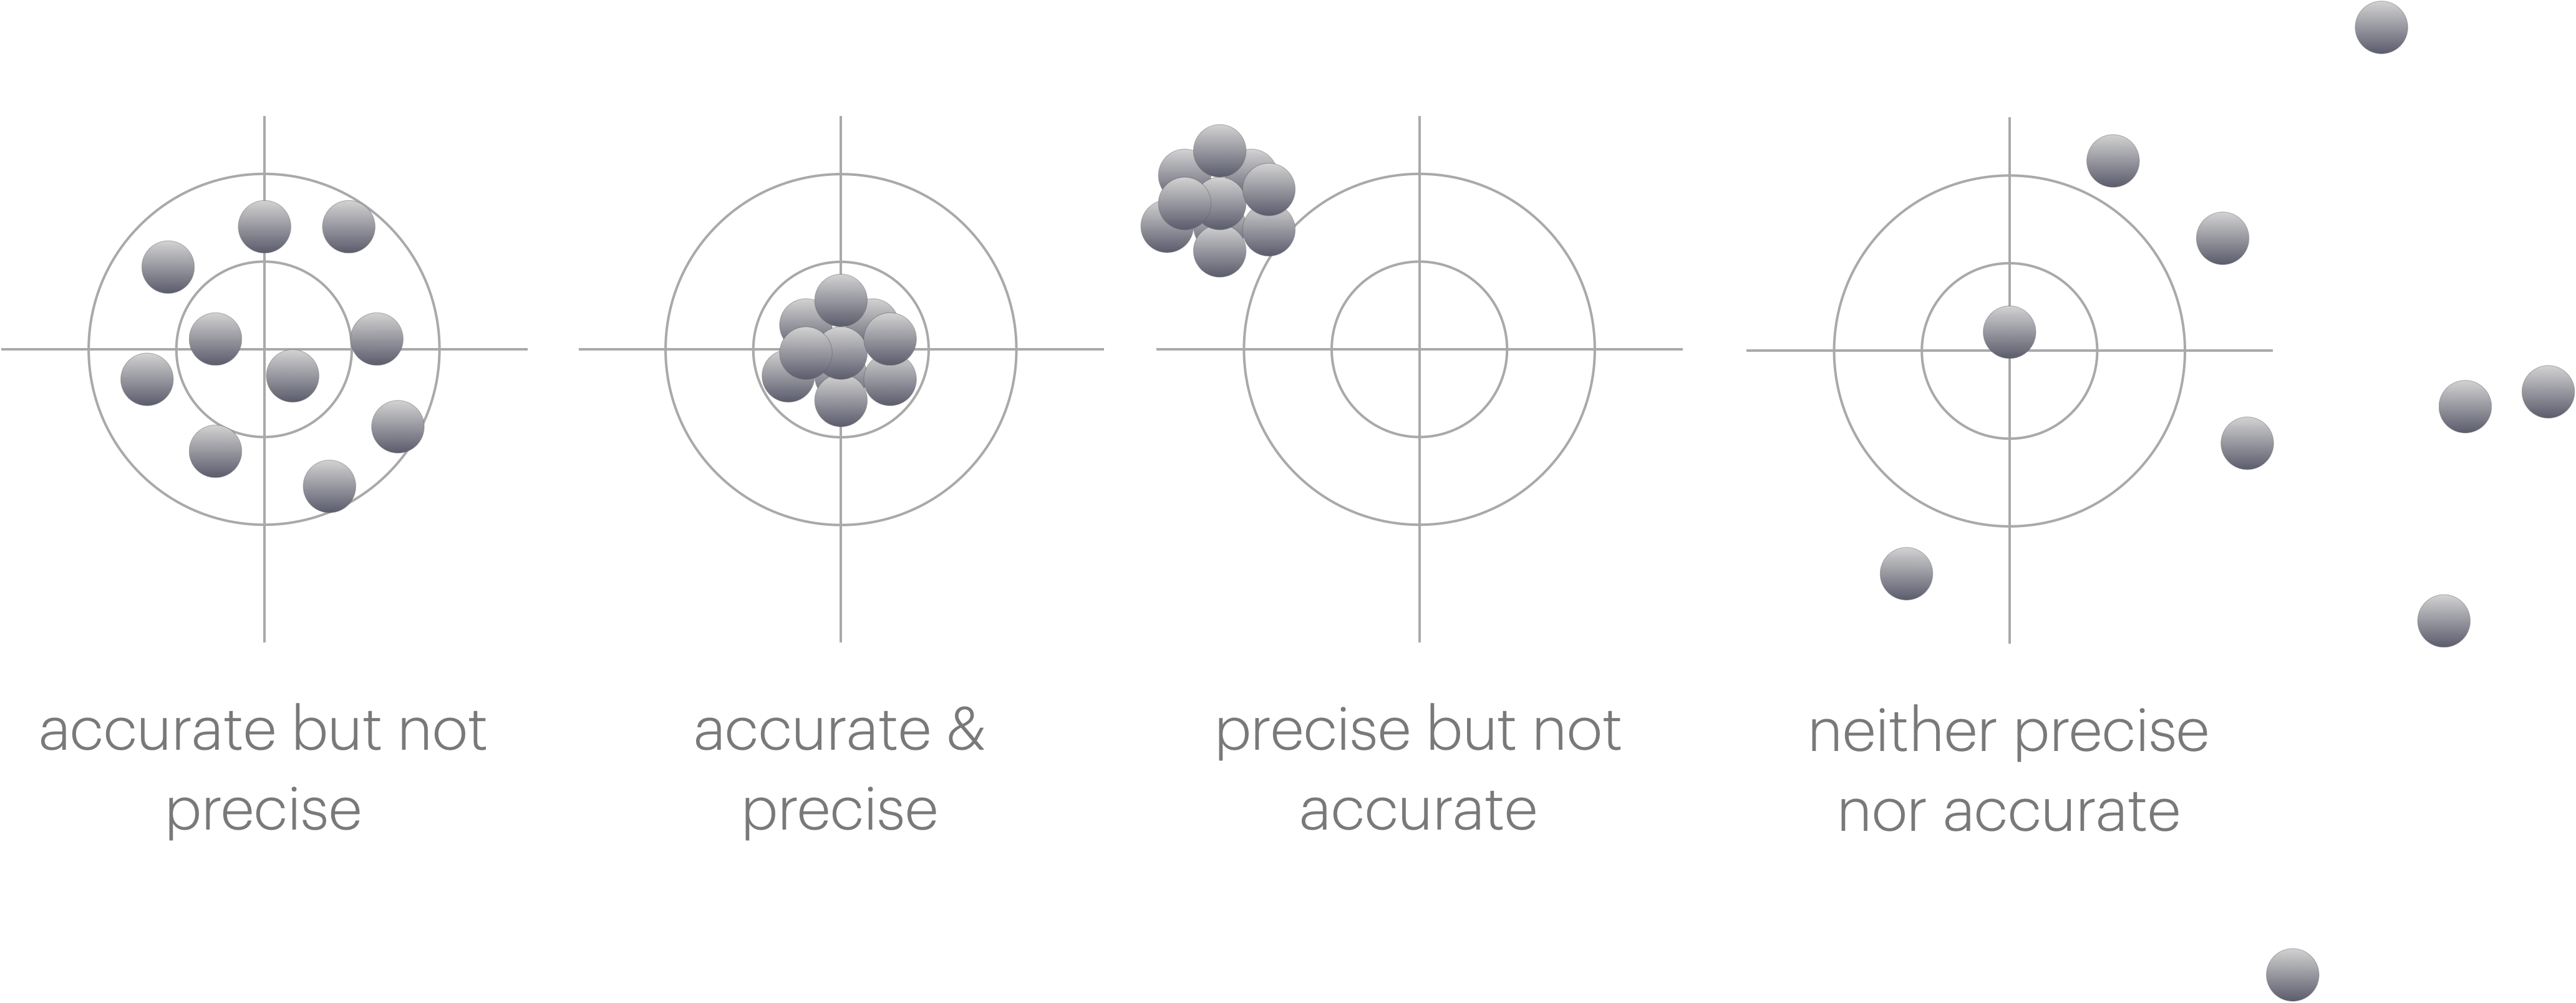
\includegraphics[keepaspectratio,alt={Four targets each showing different combinations of accuracy and precision.}]{Images/AccuracyandPrecision.png}}

}

\caption{The difference between accuracy and precision.}

\end{figure}%

When we are talking about significant figures, we are talking about
precision. The more significant figures we have, the more precise our
measurement is.

\section{Significant Figures}\label{sec-significantfigures}

Often at school you haven't really thought about significant figures,
but in science they are very important. The number of significant
figures in a measurement is a measure of how precise that measurement
is. The more significant figures, the more precise the measurement.

Therefore it is important that we don't ignore numbers which are
significant, or report values to an undue number of significant figures.

Frequently the only way you have thought about significant figures in
school is to report things like (2dp) after a value - usually because
you have trunkated the value and you want to be clear you are reporting
a trunkated value. However this is not appropriate for post school life.
Nobody has ever written 2dp or 3sf after a value in a research paper.

\begin{tcolorbox}[enhanced jigsaw, arc=.35mm, bottomrule=.15mm, bottomtitle=1mm, breakable, colback=white, colbacktitle=quarto-callout-important-color!10!white, colframe=quarto-callout-important-color-frame, coltitle=black, left=2mm, leftrule=.75mm, opacityback=0, opacitybacktitle=0.6, rightrule=.15mm, title=\textcolor{quarto-callout-important-color}{\faExclamation}\hspace{0.5em}{Don't do this!}, titlerule=0mm, toprule=.15mm, toptitle=1mm]

Never write 2dp or 3sf after a value. It is not appropriate in science
and will make you look like you don't know what you are doing.

Instead just write your answer to the correct number of significant
figures.

\end{tcolorbox}

Therefore we have to have have a way of understanding the significant
figures we have, how to report them in an appropriate way, and then we
will see in Chapter~\ref{sec-chapter2} how to use them in calculations.

\#\#\#Why we care about significant figures Significant figures are a
measure of our confidence in a value.

When we have many significant figures, we are more confident in the
value. When we have few significant figures, we are less confident in
the value.

Usually if we have any uncertaintiy in a value it is in the last
significant figure we report.

\section{How many significant figures are there?}\label{sec-howmanysf}

Like many things in science, there are rules for how to determine the
number of significant figures in a value. The rules are as follows:

\begin{tcolorbox}[enhanced jigsaw, arc=.35mm, bottomrule=.15mm, bottomtitle=1mm, breakable, colback=white, colbacktitle=quarto-callout-tip-color!10!white, colframe=quarto-callout-tip-color-frame, coltitle=black, left=2mm, leftrule=.75mm, opacityback=0, opacitybacktitle=0.6, rightrule=.15mm, title=\textcolor{quarto-callout-tip-color}{\faLightbulb}\hspace{0.5em}{Tip \ref*{tip-howmanysf}}, titlerule=0mm, toprule=.15mm, toptitle=1mm]

\quartocallouttip{tip-howmanysf} 

\begin{itemize}
\tightlist
\item
  Any non-zero digit is significant
\item
  Any 0 following a non-zero digit is significant
\item
  Any 0 to the left of the first non-zero digit is not significant
\end{itemize}

\end{tcolorbox}

By saying that any 0 after another digit we avoid ambiguity. This may be
different to what you have been taught in school.

Below are examples of numbers and how many significant figures they
have.

\begin{tcolorbox}[enhanced jigsaw, arc=.35mm, bottomrule=.15mm, bottomtitle=1mm, breakable, colback=white, colbacktitle=quarto-callout-caution-color!10!white, colframe=quarto-callout-caution-color-frame, coltitle=black, left=2mm, leftrule=.75mm, opacityback=0, opacitybacktitle=0.6, rightrule=.15mm, title=\textcolor{quarto-callout-caution-color}{\faFire}\hspace{0.5em}{How many significant figures are there?}, titlerule=0mm, toprule=.15mm, toptitle=1mm]

\(\begin{array}{cc}
123 & 3 \textrm{ sf}\\
123.4 & 4 \textrm{ sf}\\
0.123 & 3 \textrm{ sf}\\
123400 & 6 \textrm{ sf}\\
123.4 \times 10^3 & 4 \textrm{ sf}
\end{array}\)

\end{tcolorbox}

We should use standard form (or unit prefixes where appropriate) to
represent values to an appropriate precision.

\begin{tcolorbox}[enhanced jigsaw, arc=.35mm, bottomrule=.15mm, bottomtitle=1mm, breakable, colback=white, colbacktitle=quarto-callout-important-color!10!white, colframe=quarto-callout-important-color-frame, coltitle=black, left=2mm, leftrule=.75mm, opacityback=0, opacitybacktitle=0.6, rightrule=.15mm, title=\textcolor{quarto-callout-important-color}{\faExclamation}\hspace{0.5em}{Don't do this!}, titlerule=0mm, toprule=.15mm, toptitle=1mm]

Freqently in exams I will see answers such as:

\(\Delta H =\) 123854.3628 J mol\(^{-1}\)

\(\approx\) 124000 J mol\(^{-1}\) (3sf)

This latter value is actually still written to 6 significant figures.

We do not need the \(\approx\) sign as if are answer should be to three
sig figs then the answer is correct to the correct number of significant
figures.

We should write the answer with a unit prefix (or in standard form) to
avoid ambiguity.

\(\Delta H =\) 124 kJ mol\(^{-1}\)

\end{tcolorbox}

\section{Exercise on counting signficant figures}\label{sec-exercise-sf}

\section{Reading values}\label{sec-readingvalues}

When we record values in the laboratory we are limited by the precision
of the instrumentation we are using. We ususally make decisions about
equipment unconciously, for example you don't go seraching for a 4
decimal place balance to weigh out most reagents in the synthetic lab,
but you frequently do this in the physical lab.

The balances are a good place to remind us that signficant zeros matter.

There is a big diference between 0.4 g and 0.4000 g in terms of our
precision.

One thing that may be different to school is accepting that you cannot
read a scale more accurately than the scale allows.

Frequently in school you are told that if it is half way between the
graduations on a burrette then you use an increased level of precision
than the instrument allows. This is not appropriate in science.

\begin{tcolorbox}[enhanced jigsaw, arc=.35mm, bottomrule=.15mm, bottomtitle=1mm, breakable, colback=white, colbacktitle=quarto-callout-tip-color!10!white, colframe=quarto-callout-tip-color-frame, coltitle=black, left=2mm, leftrule=.75mm, opacityback=0, opacitybacktitle=0.6, rightrule=.15mm, title=\textcolor{quarto-callout-tip-color}{\faLightbulb}\hspace{0.5em}{Tip \ref*{tip-scales}}, titlerule=0mm, toprule=.15mm, toptitle=1mm]

\quartocallouttip{tip-scales} 

You cannot read a scale more accurately than the scale allows.

\end{tcolorbox}

\begin{figure}[H]

{\centering 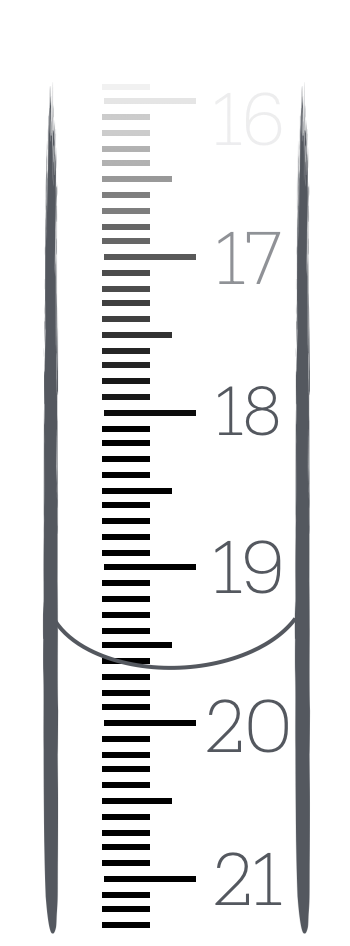
\includegraphics[width=0.3\linewidth,height=\textheight,keepaspectratio,alt={A sketch of a burette with a meniscus bottom between 19.6 and 19.7 mL. }]{Images/burette.png}

}

\caption{The limit of precision on a burette means we can only read as
accurately as the scale allows.}

\end{figure}%

In the case of the burette above, we can only read to 1 decimal place.
If the meniscus is between 19.6 and 19.7 mL, we \textbf{cannot} report
the value as 19.65 mL (as you may have been taught in school). This is
because we are adding a precision we do not have. How do we know it is
19.65 mL and not 19.66 mL or 19.64 mL? We don't. Therefore we stick with
the precision of the instrument.

In this case you either have to choose `is it closer to 19.6 mL or 19.7
mL' and report the value as either 19.6 mL or 19.7 mL or to avoid
systematic bias we \emph{round to even}.

\section{Round to even}\label{sec-roundtoeven}

If we think about rounding we need to consider the possibility of
systematic bias. If we always round up, then we will always be reporting
a value that is higher than the true value. If we always round down,
then we will always be reporting a value that is lower than the true
value.

Consider the following values which we need to report to 1 decimal
place:

\begin{tcolorbox}[enhanced jigsaw, arc=.35mm, bottomrule=.15mm, bottomtitle=1mm, breakable, colback=white, colbacktitle=quarto-callout-caution-color!10!white, colframe=quarto-callout-caution-color-frame, coltitle=black, left=2mm, leftrule=.75mm, opacityback=0, opacitybacktitle=0.6, rightrule=.15mm, title=\textcolor{quarto-callout-caution-color}{\faFire}\hspace{0.5em}{Rounding values?}, titlerule=0mm, toprule=.15mm, toptitle=1mm]

\(\begin{array}{ccc}
19.10 & 19.1 & \textrm{no rounding needed}\\
19.11 & 19.1 & \textrm{round down}\\
19.12 & 19.1 & \textrm{round down}\\
19.13 & 19.1 & \textrm{round down}\\
19.14 & 19.1 & \textrm{round down}\\
19.15 & 19.? & ???\\
19.16 & 19.2 & \textrm{round up}\\
19.17 & 19.2 & \textrm{round up}\\
19.18 & 19.2 & \textrm{round up}\\
19.19 & 19.2 & \textrm{round up}\\
19.20 & 19.2 & \textrm{no rounding needed}  \\
\end{array}\)

\end{tcolorbox}

If we always round the value ending in a 5 up (as you maybe always have
before) then we have more values rounding up than we have rounding ndown
and we introduce a slight systematic bias increasing our value over all.

Therefore if a value ends exactly in a 5 and needs to be rounded we
instead `round to even', which should mean that half of the time it will
round up and half of the time it rounds down.

\begin{tcolorbox}[enhanced jigsaw, arc=.35mm, bottomrule=.15mm, bottomtitle=1mm, breakable, colback=white, colbacktitle=quarto-callout-tip-color!10!white, colframe=quarto-callout-tip-color-frame, coltitle=black, left=2mm, leftrule=.75mm, opacityback=0, opacitybacktitle=0.6, rightrule=.15mm, title=\textcolor{quarto-callout-tip-color}{\faLightbulb}\hspace{0.5em}{Tip \ref*{tip-roundtoeven}}, titlerule=0mm, toprule=.15mm, toptitle=1mm]

\quartocallouttip{tip-roundtoeven} 

If a value ends in a 5 exactly and needs rounding we should round to the
nearest even number.

\end{tcolorbox}

\begin{tcolorbox}[enhanced jigsaw, arc=.35mm, bottomrule=.15mm, bottomtitle=1mm, breakable, colback=white, colbacktitle=quarto-callout-caution-color!10!white, colframe=quarto-callout-caution-color-frame, coltitle=black, left=2mm, leftrule=.75mm, opacityback=0, opacitybacktitle=0.6, rightrule=.15mm, title=\textcolor{quarto-callout-caution-color}{\faFire}\hspace{0.5em}{Examples of rounding to even.}, titlerule=0mm, toprule=.15mm, toptitle=1mm]

If each of the following should be reported to 3 significant figures

\(\begin{array}{cccc}
47.58 & \textrm{rounds up to} & 47.6 &\\
8.325 & \textrm{rounds down to} & 8.32 & \textrm{rounded to even}\\
3.621 & \textrm{rounds down to} & 3.62 &\\
64.55 & \textrm{rounds up to} & 64.6 & \textrm{rounded to even}\\
10.050003 & \textrm{rounds up to} & 10.5 &\\
\end{array}\)

\end{tcolorbox}

\section{Self assessment exercises}\label{self-assessment-exercises}

\subsection{Self check on our learning so far.}\label{sec-SelfcheckSF}

\begin{tcolorbox}[enhanced jigsaw, arc=.35mm, bottomrule=.15mm, bottomtitle=1mm, breakable, colback=white, colbacktitle=quarto-callout-note-color!10!white, colframe=quarto-callout-note-color-frame, coltitle=black, left=2mm, leftrule=.75mm, opacityback=0, opacitybacktitle=0.6, rightrule=.15mm, title=\textcolor{quarto-callout-note-color}{\faInfo}\hspace{0.5em}{What is 16453 rounded to 2 significant figures?}, titlerule=0mm, toprule=.15mm, toptitle=1mm]

16 \(\times\) 10\(^3\)

Any number we write is considered significant so we can't write 16000
and think it is 2 significant figures. We need to use standard form to
avoid ambiguity.

\end{tcolorbox}

\begin{tcolorbox}[enhanced jigsaw, arc=.35mm, bottomrule=.15mm, bottomtitle=1mm, breakable, colback=white, colbacktitle=quarto-callout-note-color!10!white, colframe=quarto-callout-note-color-frame, coltitle=black, left=2mm, leftrule=.75mm, opacityback=0, opacitybacktitle=0.6, rightrule=.15mm, title=\textcolor{quarto-callout-note-color}{\faInfo}\hspace{0.5em}{What is 0.090305 rounded to 2 significant figures?}, titlerule=0mm, toprule=.15mm, toptitle=1mm]

0.090

It is easy to forget significant zeros after our first non-zero digit.
In this case we have 2 significant figures, the 9 and the 0 after it.

\end{tcolorbox}

\begin{tcolorbox}[enhanced jigsaw, arc=.35mm, bottomrule=.15mm, bottomtitle=1mm, breakable, colback=white, colbacktitle=quarto-callout-note-color!10!white, colframe=quarto-callout-note-color-frame, coltitle=black, left=2mm, leftrule=.75mm, opacityback=0, opacitybacktitle=0.6, rightrule=.15mm, title=\textcolor{quarto-callout-note-color}{\faInfo}\hspace{0.5em}{What is 2.4503 rounded to 2 significant figures?}, titlerule=0mm, toprule=.15mm, toptitle=1mm]

2.5

In this case round to even doesn't apply as it isn't exactly `5'.

\end{tcolorbox}

\begin{tcolorbox}[enhanced jigsaw, arc=.35mm, bottomrule=.15mm, bottomtitle=1mm, breakable, colback=white, colbacktitle=quarto-callout-note-color!10!white, colframe=quarto-callout-note-color-frame, coltitle=black, left=2mm, leftrule=.75mm, opacityback=0, opacitybacktitle=0.6, rightrule=.15mm, title=\textcolor{quarto-callout-note-color}{\faInfo}\hspace{0.5em}{What is 37.4500 rounded to 3 significant figures?}, titlerule=0mm, toprule=.15mm, toptitle=1mm]

37.4

In this case round to even does apply as it is a 5 we are having to
round.

\end{tcolorbox}

\subsection{Self assessment exercise: Write the following values to the
listed sf.}\label{sec-SAQroundtoeven}

\bookmarksetup{startatroot}

\chapter{The use of the correct number of significant figures in
calculations.}\label{sec-chapter2}

In Chapter~\ref{sec-chapter1} we have learnt about significant figures
and why they are important in understanding the confidence we have in a
value.

Now we need to learn the rules to how many significant figures we should
use after doing calculations.

There are different rules for how we handle significant figures
depending upon the type of calculation we have done. Freqently we may
have more than one step in a calculation, and therefore we need to be
concious of the appropriate significant figures in each step.

\section{Significant figures in addition and
subtraction}\label{sec-sfaddsub}

When adding or subtracting values, the number of decimal places in the
result should be the same as the value with the least number of decimal
places in your calculation.

We cannot add precision, I can't measure something with a meter rule
with 1 cm increments, a 15 cm rule with 1 mm increments and a micrometer
with 1 μm increments and then add them together and expect to have a
result with 1 μm precision. The result will be limited by the least
precise measurement.

\begin{tcolorbox}[enhanced jigsaw, arc=.35mm, bottomrule=.15mm, bottomtitle=1mm, breakable, colback=white, colbacktitle=quarto-callout-tip-color!10!white, colframe=quarto-callout-tip-color-frame, coltitle=black, left=2mm, leftrule=.75mm, opacityback=0, opacitybacktitle=0.6, rightrule=.15mm, title=\textcolor{quarto-callout-tip-color}{\faLightbulb}\hspace{0.5em}{Tip \ref*{tip-scales}: Significant figures in addition and subtraction.}, titlerule=0mm, toprule=.15mm, toptitle=1mm]

\quartocallouttip{tip-scales} 

When adding or subtracting values, the number of decimal places in the
result should be the same as the value with the least number of decimal
places in your calculation.

\end{tcolorbox}

\begin{tcolorbox}[enhanced jigsaw, arc=.35mm, bottomrule=.15mm, bottomtitle=1mm, breakable, colback=white, colbacktitle=quarto-callout-caution-color!10!white, colframe=quarto-callout-caution-color-frame, coltitle=black, left=2mm, leftrule=.75mm, opacityback=0, opacitybacktitle=0.6, rightrule=.15mm, title=\textcolor{quarto-callout-caution-color}{\faFire}\hspace{0.5em}{Examples of significant figures in addition and subtraction.}, titlerule=0mm, toprule=.15mm, toptitle=1mm]

\begin{itemize}
\tightlist
\item
  Convert 20 ºC to Kelvin.
\end{itemize}

We know our measured temperature to 0 decimal places, therefore our
answer should be to 0 decimal places.

T = 20 ºC + 273.15 K = 293 K

\begin{itemize}
\tightlist
\item
  An ideal gas was heated with 1.75 kJ of energy an allowed to do 250 J
  of work. What is the change in internal energy of the gas?
\end{itemize}

In this case we have different units, so if we convert 250 J to kJ we
have 0.250 kJ. The least number of decimal places is 2, therefore our
answer should be to 2 decimal places.

\(\Delta U = 1.75 \textrm{ kJ} - 0.250 \textrm{ kJ} = 1.50 \textrm{ kJ}\)

This unit conversion kJ to J (or vice versa) is common in thermodynamics
calculations where \(\Delta H\) is usually reported in kJ mol\(^{-1}\),
but \(\Delta S\) is usually reported in J K mol\(^{-1}\).

It is easy to forget the significant zero at the end of this number as
usually our calculator will not report it, but including it gives us our
answer to a higher, more appropriate, precision.

\end{tcolorbox}

\subsection{Exercises with addition and subtraction
examples.}\label{exercises-with-addition-and-subtraction-examples.}

\subsubsection{Self check on our learning so
far.}\label{sec-SelfcheckSFaddsub}

\begin{tcolorbox}[enhanced jigsaw, arc=.35mm, bottomrule=.15mm, bottomtitle=1mm, breakable, colback=white, colbacktitle=quarto-callout-note-color!10!white, colframe=quarto-callout-note-color-frame, coltitle=black, left=2mm, leftrule=.75mm, opacityback=0, opacitybacktitle=0.6, rightrule=.15mm, title=\textcolor{quarto-callout-note-color}{\faInfo}\hspace{0.5em}{What is 15.4 g + 0.16 g to the correct number of significant figures?}, titlerule=0mm, toprule=.15mm, toptitle=1mm]

15.6 g

The rule for adding and subtracting is that the answer should be
reported to the least number of decimal places in the calculation. In
this case 15.4 g has 1 decimal place, and 0.16 g has 2 decimal places,
so our answer should be reported to 1 decimal place.

\end{tcolorbox}

\begin{tcolorbox}[enhanced jigsaw, arc=.35mm, bottomrule=.15mm, bottomtitle=1mm, breakable, colback=white, colbacktitle=quarto-callout-note-color!10!white, colframe=quarto-callout-note-color-frame, coltitle=black, left=2mm, leftrule=.75mm, opacityback=0, opacitybacktitle=0.6, rightrule=.15mm, title=\textcolor{quarto-callout-note-color}{\faInfo}\hspace{0.5em}{What is -154.3 kJ mol\(^{-1}\) + 894.2 J mol\(^{-1}\) to the correct
number of significant figures?}, titlerule=0mm, toprule=.15mm, toptitle=1mm]

-153.4 kJ mol\(^{-1}\)

Here we have different units, so if we convert 894.2 J mol\(^{-1}\) to
kJ mol\(^{-1}\) we have 0.8942 kJ mol\(^{-1}\).

Now we can compare the number of decimal places in each value. -154.3 kJ
mol\(^{-1}\) has 1 decimal place, and 0.8942 kJ mol\(^{-1}\) has 4
decimal places, so keeping the fewest decimal places, our answer should
be reported to 1 decimal place.

\end{tcolorbox}

The following are molar masses of some common elements. Use these values
to answer the following questions.

\begin{longtable}[]{@{}cc@{}}
\caption{A selection of atomic masses of common
elements.}\label{tbl-atomicmassescommon}\tabularnewline
\toprule\noalign{}
& \(R_A\) / g mol\(^{-1}\) \\
\midrule\noalign{}
\endfirsthead
\toprule\noalign{}
& \(R_A\) / g mol\(^{-1}\) \\
\midrule\noalign{}
\endhead
\bottomrule\noalign{}
\endlastfoot
H & 1.00794 \\
C & 12.011 \\
O & 15.9994 \\
N & 14.0067 \\
Cl & 35.45 \\
\end{longtable}

\begin{tcolorbox}[enhanced jigsaw, arc=.35mm, bottomrule=.15mm, bottomtitle=1mm, breakable, colback=white, colbacktitle=quarto-callout-note-color!10!white, colframe=quarto-callout-note-color-frame, coltitle=black, left=2mm, leftrule=.75mm, opacityback=0, opacitybacktitle=0.6, rightrule=.15mm, title=\textcolor{quarto-callout-note-color}{\faInfo}\hspace{0.5em}{What is the molar mass of HCl to the correct number of significant
figures?}, titlerule=0mm, toprule=.15mm, toptitle=1mm]

36.46 g mol\(^{-1}\)

35.45 g mol\(^{-1}\) + 1.00794 g mol\(^{-1}\) = \st{36.45794 g
mol}\(^{-1}\) = 36.46 g mol\(^{-1}\)

Cl has the least number of decimal places (2), so our answer should only
be reported to 2 decimal places.

\end{tcolorbox}

Given we should now be in the habit of reporting our answers to the
correct number of significant figures, this is no longer going to be
asked in the following exercises, but we should still be concious of the
number of significant figures in our answers.

\begin{tcolorbox}[enhanced jigsaw, arc=.35mm, bottomrule=.15mm, bottomtitle=1mm, breakable, colback=white, colbacktitle=quarto-callout-note-color!10!white, colframe=quarto-callout-note-color-frame, coltitle=black, left=2mm, leftrule=.75mm, opacityback=0, opacitybacktitle=0.6, rightrule=.15mm, title=\textcolor{quarto-callout-note-color}{\faInfo}\hspace{0.5em}{What is the molar mass of C\(_2\)H\(_5\)OH?}, titlerule=0mm, toprule=.15mm, toptitle=1mm]

46.064 g mol\(^{-1}\)

Carbon's molar mass has 3 decimal places, hydrogen's molar mass has 5
decimal places and oxygen's molar mass has 4 decimal places.

In addition questions our answer should be reported to the fewest
decimal places, which in this case is 3.

\end{tcolorbox}

\begin{tcolorbox}[enhanced jigsaw, arc=.35mm, bottomrule=.15mm, bottomtitle=1mm, breakable, colback=white, colbacktitle=quarto-callout-note-color!10!white, colframe=quarto-callout-note-color-frame, coltitle=black, left=2mm, leftrule=.75mm, opacityback=0, opacitybacktitle=0.6, rightrule=.15mm, title=\textcolor{quarto-callout-note-color}{\faInfo}\hspace{0.5em}{What is the molar mass of C\(_6\)H\(_{12}\)O\(_6\)?}, titlerule=0mm, toprule=.15mm, toptitle=1mm]

180.158 g mol\(^{-1}\)

Once you get used to the idea of handling signficant figures you will be
able to perform your calculations, then correct your values to the
correct number of significant figures when reporting.

Here Carbon has 3 decimal places, so the answer should be reported to 3
decimal places, even if the value coming from a calculator would be
180.15768.

\end{tcolorbox}

\begin{tcolorbox}[enhanced jigsaw, arc=.35mm, bottomrule=.15mm, bottomtitle=1mm, breakable, colback=white, colbacktitle=quarto-callout-note-color!10!white, colframe=quarto-callout-note-color-frame, coltitle=black, left=2mm, leftrule=.75mm, opacityback=0, opacitybacktitle=0.6, rightrule=.15mm, title=\textcolor{quarto-callout-note-color}{\faInfo}\hspace{0.5em}{What is the molar mass of C\(_{12}\)H\(_8\)N\(_2\)?}, titlerule=0mm, toprule=.15mm, toptitle=1mm]

180.209 g mol\(^{-1}\)

Again carbon limits the number of decimal places to give in our answer.

\end{tcolorbox}

\begin{tcolorbox}[enhanced jigsaw, arc=.35mm, bottomrule=.15mm, bottomtitle=1mm, breakable, colback=white, colbacktitle=quarto-callout-note-color!10!white, colframe=quarto-callout-note-color-frame, coltitle=black, left=2mm, leftrule=.75mm, opacityback=0, opacitybacktitle=0.6, rightrule=.15mm, title=\textcolor{quarto-callout-note-color}{\faInfo}\hspace{0.5em}{What is the molar mass of C\(_{12}\)H\(_{22}\)O\(_{11}\)?}, titlerule=0mm, toprule=.15mm, toptitle=1mm]

342.300 g mol\(^{-1}\)

It is important to remember to include significant zeros if they are
there. These are easy to remember because there were non zero numbers
after them, but remember to write them down.

\end{tcolorbox}

\subsubsection{Self assessment question on significant figures in
addition and
subtraction.}\label{self-assessment-question-on-significant-figures-in-addition-and-subtraction.}

Please remember you can refresh this question.

\section{Significant figures in multiplication and
division}\label{sec-sfmuldiv}

When multiplying or dividing values, the number of significant figures
in the result should be the same as the value with the least number of
significant figures in your calculation.

First we need to quickly count the number of significant figures in each
value. If we have a unit conversion (such as mm to cm) then this is
`exact' and does not change the number of significant figures in our
value. Some unit conversions have limited significant figures, others
are precise. In either case it is always a good habit to use more
significant figures in constants than in our other values.

\begin{tcolorbox}[enhanced jigsaw, arc=.35mm, bottomrule=.15mm, bottomtitle=1mm, breakable, colback=white, colbacktitle=quarto-callout-tip-color!10!white, colframe=quarto-callout-tip-color-frame, coltitle=black, left=2mm, leftrule=.75mm, opacityback=0, opacitybacktitle=0.6, rightrule=.15mm, title=\textcolor{quarto-callout-tip-color}{\faLightbulb}\hspace{0.5em}{Tip \ref*{tip-scales}: Significant figures in multiplication and division.}, titlerule=0mm, toprule=.15mm, toptitle=1mm]

\quartocallouttip{tip-scales} 

When multiplying or dividing values, the number of significant figures
in the result should be the same as the value with the least number of
significant figures in your calculation.

\end{tcolorbox}

\begin{tcolorbox}[enhanced jigsaw, arc=.35mm, bottomrule=.15mm, bottomtitle=1mm, breakable, colback=white, colbacktitle=quarto-callout-caution-color!10!white, colframe=quarto-callout-caution-color-frame, coltitle=black, left=2mm, leftrule=.75mm, opacityback=0, opacitybacktitle=0.6, rightrule=.15mm, title=\textcolor{quarto-callout-caution-color}{\faFire}\hspace{0.5em}{Example of significant figures in multiplication and division - the
ideal gas law.}, titlerule=0mm, toprule=.15mm, toptitle=1mm]

\begin{itemize}
\tightlist
\item
  Determine the number of moles of gas in a cylinder with a volume of
  exactly 2.52 L at a pressure of 50.24 bar and a temperature of 273 K.
\end{itemize}

Here we need to do a couple of unit conversions to get our values into
base SI units.

The volume is already in L, which is a derived unit, but we need to
convert it to m\(^3\). 1 L \(\equiv\) 1 dm\(^3\) = 1 x 10\(^{-3}\)
m\(^3\), so we have 2.52 L = 2.52 x 10\(^{-3}\) m\(^3\). This is an
exact conversion, so the number of significant figures in our value does
not change. Recall that the volume is described as ``exactly'' 2.52 L,
so we have `infinite' significant figures in our volume.

The pressure is in bar, which is not an SI unit, so we need to convert
it to Pa. 1 bar = 1 x 10\(^5\) Pa, so we have 50.24 bar = 5.024 x
10\(^6\) Pa. This is also an exact conversion. The pressure has 4
significant figures, so our pressure in bar will also have 4 significant
figures.

Using the ideal gas law, we can calculate the number of moles of gas in
the cylinder.

\(pV = nRT\) so \(n = \frac{pV}{RT}\)

Putting in our values:

\[n = \frac{5.024 \times 10^6 \textrm{ Pa} \times 2.52 \times 10^{-3} \textrm{ m}^3}{8.31446 \textrm{ J K}^{-1} \textrm{ mol}^{-1} \times 273 \textrm{ K}}\]

\(n = 5.58 \textrm{ mol}\)

Temperature only has 3 significant figures, so our answer should be
reported to 3 significant figures.

\end{tcolorbox}

\begin{tcolorbox}[enhanced jigsaw, arc=.35mm, bottomrule=.15mm, bottomtitle=1mm, breakable, colback=white, colbacktitle=quarto-callout-caution-color!10!white, colframe=quarto-callout-caution-color-frame, coltitle=black, left=2mm, leftrule=.75mm, opacityback=0, opacitybacktitle=0.6, rightrule=.15mm, title=\textcolor{quarto-callout-caution-color}{\faFire}\hspace{0.5em}{Example of significant figures in multiplication and division - heat
capacity.}, titlerule=0mm, toprule=.15mm, toptitle=1mm]

\begin{itemize}
\tightlist
\item
  Determine the energy put into a system when a 1.000 kg block of copper
  is heated from 20.16 ºC to 60.52 ºC. The specific heat capacity of
  copper is 385 J kg\(^{-1}\) K\(^{-1}\).
\end{itemize}

We can calculate the energy put into the system using the equation:

\(q = m c \Delta T\)

First we need to determine the change in temperature, \(\Delta T\).

\(\Delta T = T_{\textrm{final}} - T_{\textrm{initial}}\)

\(\Delta T = 60.52 ºC - 20.16 ºC = 40.36 ºC\)

We've followed the rules for addition and subtraction, so our answer has
2 decimal places, which is the same as the least number of decimal
places in our calculation.

Now we can calculate the energy put into the system, \(q\).

\(q = 1.000 \textrm{ kg} \times 385 \textrm{ J kg}^{-1} \textrm{ K}^{-1} \times 40.36 \textrm{ K}\)

The mass has 4 significant figures, the specific heat capacity has 3
significant figures, and the temperature change has 4 significant
figures. The least number of significant figures in our calculation is
3, so our answer should be reported to 3 significant figures.

\(q = 15.5 \textrm{ kJ}\)

Note: I've changed my units to kJ to make reporting to 3 significant
figures easier. If I had left my answer in J, I would have reported it
as 15.5 \(\times\) 10³ J, which is not as clear (and is more to type).

\end{tcolorbox}

\section{Exercises with multiplication and division
examples.}\label{exercises-with-multiplication-and-division-examples.}

\subsection{Self check on our learning so
far.}\label{sec-SelfcheckSFmultdiv}

\begin{tcolorbox}[enhanced jigsaw, arc=.35mm, bottomrule=.15mm, bottomtitle=1mm, breakable, colback=white, colbacktitle=quarto-callout-note-color!10!white, colframe=quarto-callout-note-color-frame, coltitle=black, left=2mm, leftrule=.75mm, opacityback=0, opacitybacktitle=0.6, rightrule=.15mm, title=\textcolor{quarto-callout-note-color}{\faInfo}\hspace{0.5em}{If each side of a rectangle was measured to be 2.34 cm and 1.2 cm, what
is the area?}, titlerule=0mm, toprule=.15mm, toptitle=1mm]

A = 2.8 cm\(^2\)

The area of a rectangle is given by \(A = l \times w\), so from our
calculator we get a value of 2.808 cm\(^2\). Since one of our sides only
has 2 significant figures, using our rule of using the fewest
significant figures, our answer should be reported to 2 significant
figures.

\end{tcolorbox}

\begin{tcolorbox}[enhanced jigsaw, arc=.35mm, bottomrule=.15mm, bottomtitle=1mm, breakable, colback=white, colbacktitle=quarto-callout-note-color!10!white, colframe=quarto-callout-note-color-frame, coltitle=black, left=2mm, leftrule=.75mm, opacityback=0, opacitybacktitle=0.6, rightrule=.15mm, title=\textcolor{quarto-callout-note-color}{\faInfo}\hspace{0.5em}{What is the volume of a cylinder with a diameter of 2.3 cm and a height
of 12.4 cm?}, titlerule=0mm, toprule=.15mm, toptitle=1mm]

V = 52 cm\(^3\)

On the surface this is an easy calculation following our rules of
significant figures we retain the fewest significant figures in our
answer, which is 2.

You might be tempted to use the radius of the circle, and `half' the
diameter, but in doing this we can get into a mess with our significant
figures because we can't gain significant figures by dividing by 2.

Instead we can use the diameter directly in our calculation,
\(V = \frac{\pi d^2 h}{4}\) which simplifies the significant figure
handling.

This shows that is is often easiest to use algebraic rearrangements to
avoid having to do extra calculations which may introduce complications
in our consideration of significant figures.

\end{tcolorbox}

\begin{tcolorbox}[enhanced jigsaw, arc=.35mm, bottomrule=.15mm, bottomtitle=1mm, breakable, colback=white, colbacktitle=quarto-callout-note-color!10!white, colframe=quarto-callout-note-color-frame, coltitle=black, left=2mm, leftrule=.75mm, opacityback=0, opacitybacktitle=0.6, rightrule=.15mm, title=\textcolor{quarto-callout-note-color}{\faInfo}\hspace{0.5em}{Determine the rate constant of diffusion, \(k_d\) at 278 K, if the
viscosity of the medium, \(\eta\), is 1.518 mPa s, given \$k\_d =
\frac{8RT}{3\eta}.}, titlerule=0mm, toprule=.15mm, toptitle=1mm]

\(k_d = 4.06 \times 10^{6}\) m\(^3\) s\(^{-1}\) = 4.06 \times 10\(^{9}\)
dm\(^3\) s\(^{-1}\)

This is a more challenging question as you won't hve come across this
equation before, but the principles are the same. This is a
multiplication and division question, so we need to consider the number
of significant figures in each value, and report our answer to the
fewest number of significant figures in our calculation.

The integers, 8 and 3 are exact values, so can be considered to have
infinite significant figures.

When values are large some poeple want to write 4 060 000 (3sf) but
given our rule that if you write a digit it is significant this answer
is actually 7 significant figures.

\end{tcolorbox}

\section{Significant figures in logarithms}\label{sec-sflog}

Significant figures in logs and lns are a little different to the rules
for addition, subtraction, multiplication and division because we have
to think about the `value' when accounting for how many significant
figures we have in our answer.

\begin{tcolorbox}[enhanced jigsaw, arc=.35mm, bottomrule=.15mm, bottomtitle=1mm, breakable, colback=white, colbacktitle=quarto-callout-tip-color!10!white, colframe=quarto-callout-tip-color-frame, coltitle=black, left=2mm, leftrule=.75mm, opacityback=0, opacitybacktitle=0.6, rightrule=.15mm, title=\textcolor{quarto-callout-tip-color}{\faLightbulb}\hspace{0.5em}{Tip \ref*{tip-scales}: Significant figures in logs and lns.}, titlerule=0mm, toprule=.15mm, toptitle=1mm]

\quartocallouttip{tip-scales} 

When taking logs we usually gain 1 significant figure, however if the
`logged value' is between 1 and the base then we do not gain a
significant figure.

\end{tcolorbox}

Practically what does this mean? and why the do we sometimes gain a
significant figure? The following example using \(\log_{10}\) will help
to explain this.

\begin{tcolorbox}[enhanced jigsaw, arc=.35mm, bottomrule=.15mm, bottomtitle=1mm, breakable, colback=white, colbacktitle=quarto-callout-caution-color!10!white, colframe=quarto-callout-caution-color-frame, coltitle=black, left=2mm, leftrule=.75mm, opacityback=0, opacitybacktitle=0.6, rightrule=.15mm, title=\textcolor{quarto-callout-caution-color}{\faFire}\hspace{0.5em}{Example of significant figures in logs and lns.}, titlerule=0mm, toprule=.15mm, toptitle=1mm]

Determine \(\log (2.234)\), \(\log(22.34)\) and \(\log(223.4)\) to the
correct number of significant figures.

Our first example is \(\log(2.234)\). The value of \(\log(2.234)\) is
0.3490831688\ldots.

The value we are taking the log of has 4 significant figures, so our
answer should have 4 significant figures. Therefore we report our answer
as 0.3491.

Now, if I take the log of 22.34 I can also write this as
\(\log(2.234 \times 10^1)\).

Using our `rules of logs', we can write this as
\(\log(2.234) + \log(10^1) = 0.3491 + 1 = 1.3491\).

Since our value of \(\log(10^1)\) is an exact value, it can be
considered to have infinite significant figures, and we can add these
values according to the rules in Section~\ref{sec-sfaddsub}.

Finally, if I take the log of 223.4 I can also write this as
\(\log(2.234 \times 10^2)\). The value we are taking the log of has 4
significant figures, so our answer should have 4 significant figures.
Therefore we report our answer as 2.3491.

You can see why we gain a significant figure when taking the log of a
value greater than 10, but not when taking the log of a value less than
10. The `value' of the number we are taking the log of is important in
determining how many significant figures we have in our answer.

The same principle works if we have very small numbers, for example
\(\log(0.002234)\) which we can write as
\(\log(2.234 \times 10^{-3}) = \log(2.234) + \log(10^{-3}) = 0.3491 - 3 = -2.6509\).

\end{tcolorbox}

\bookmarksetup{startatroot}

\chapter{}\label{section}

\bookmarksetup{startatroot}

\chapter{}\label{section-1}




\end{document}
